The conic parameters for the given curve are
% The general equation is given as,
% \begin{align}\label{4/4/eq:eq2}
% \vec{x}^\top \textbf{V} \textbf{x} + 2 \vec{u}^\top \textbf{x} + f = 0 
% \end{align}
% Comparing \eqref{4/4/eq:eq1} and \eqref{4/4/eq:eq2} we get,
\begin{align}\label{4/4/eq:eq3}
\vec{V} = \myvec{1 & 0\\0 & 1} ,
\vec{u} = \myvec{-2\\0} , 
f = 3
\end{align}
The center of circle is 
\begin{align}\label{4/4/eq:eq4}
\vec{c} &= -  \vec{u}
&= \myvec{2\\0} 
\end{align}
The radius of the circle is
\begin{align}\label{4/4/eq:eq6}
r &= \sqrt{\vec{u}^\top \vec{u} -f}
&= 1 \text{ unit}
\end{align}
This is verified in Fig. \ref{4/4/Fig:1}
\begin{figure}[h]
%
\centering
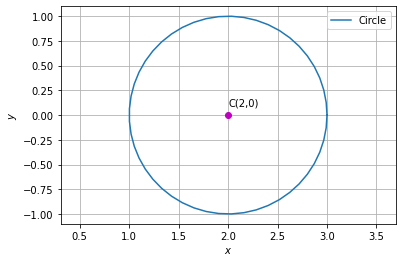
\includegraphics[width=\columnwidth]{solutions/4/4/image.png}
\caption{Plot obtained from Python code}
\label{4/4/Fig:1}
\end{figure}
